\chapter{SCADA systémy}
\label{scada}
\tab V tejto kapitole je uvedený teoretický základ o internete vecí (IoT - Internet of Things), jeho výhody a nevýhody. Podrobnejšie je popísané využitie v priemysle, tzv. SCADA systémy a komunikačné protokoly pomocou ktorých jednotlivé zariadenia v sieti komunikujú.
\section{Základný prehľad IoT}
\tab Internet vecí je dnes veľmi aktuálna téma. Ide o sieť zariadení (príručné zariadenia, vozidlá, domáce spotrebiče, a pod.) ktoré sú vybavené elektronikou, rôznymi senzormi a sieťovou konektivitou, ktorá umožňuje vzájomné prepojenie a výmenu dát medzi týmito zariadeniami. Ide o komunikáciu tzv. inteligentných (smart) zariadení cez internet. Prepojenie je väčšinou bezdrôtové, cez Wi-Fi, alebo Bluetooth. Internet vecí umožňuje vzdialené snímanie, alebo riadenie v rámci celej sieťovej infraštruktúry. Umožňuje to tak užívateľom dosiahnuť väčšiu automatizáciu, lepšiu analýzu a integráciu v rámci celého systému. Internet vecí môže mať spotrebiteľské využitie, napr. v chytrej domácnosti (smart home), kde sú jednotlivé domáce spotrebiče vzájomne prepojené cez Wi-Fi a užívateľ môže centrálne ovládať všetky svoje zariadenia. Internet vecí má ale hlavne podnikové využitie, prevažne z dôvodov zvýšenia automatizácie a úspory nákladov na prevádzku\cite{IoTFundamentals}. \newline\newline
\textbf{Výhody internetu vecí sú:}
\begin{itemize}
\item Čas - jednotlivé zariadenia, snímače a riadiace prvky nám šetria veľké množstvo času. Údaje je možné sledovať a riadiť na diaľku, bez nutnosti neustáleho cestovania na konkrétne miesta a ručného zapisovania údajov
\item Peniaze - možnosť vzdialeného prístupu a riadenia taktiež šetrí veľké množstvo financií, je potrebný menší počet zamestnancov
\item Zariadenia nám poskytujú presnejšie analýzy a dáta, bez nutnosti zásahu ľudského faktoru
\item Sledovanie - automatické sledovanie hodnôt, pripomienok a pod.
\end{itemize}
\textbf{Nevýhody sú:}
\begin{itemize}
\item Bezpečnosť - bezpečnosť je veľký problém v internete vecí. Dáta v zariadeniach musia byť dôkladne zašifrované. Zariadenia totiž môžu obsahovať osobné informácie o užívateľoch, ktoré môžu byť zneužité. Jednotlivé siete sú taktiež náchylné k rôznym útokom, prípadne môžu byť napadnuté a použité pri útoku samotnom, napr. rôzne DDoS útoky
\item Nekompatibilita - jednotlivé zariadenia nemusia spolu navzájom komunikovať, napr. ak každé zariadenie používa komunikačné protokoly vytvorené svojím výrobcom\cite{IoTFundamentals}
\end{itemize}
\section{SCADA systémy}
\tab Vo svojej práci sa budem bližšie venovať priemyselnému využitiu internetu vecí, konkrétne tzv. SCADA systémom. SCADA (Supervisory Control And Data Acquisition) systém je typ architektúry riadiaceho systému využívajúceho počítače, sieťové prepojenie a rôzne vzdialene riadené objekty. SCADA systémy sú využívané prevažne v rôznych výrobných (výrobné linky, baliace linky, skladové systémy) a energetických (elektrárne, teplárne, výmenníkové stanice) závodoch, ale aj v technológiach budov (vzduchotechnika, zabezpečenie, dochádzkové systémy) a v ekológií (emisný monitoring, čističky odpadných vôd). V Českej republike sú SCADA systémy využívané napríklad spoločnosťami ako RWE, E.ON alebo skupinou ČEZ. \par 
SCADA systémy sa radia medzi tzv. OT (Operational Technology) siete. Na rozdiel od bežných IT sietí, ktoré slúžia hlavne na prepojenie zariadení cez internet, OT siete slúžia na monitorovanie a riadenie zariadení v rôznych priemyselných odvetviach. Čo sa bezpečnosti týka, IT siete sa zameriavajú hlavne na dôkladnú autentizáciu jednotlivých zariadení, zatiaľ čo v OT sieťach ide do popredia fyzická ochrana systému. OT siete sú väčšinou izolované od bežnej TCP/IP prevádzky a využívajú proprietárne protokoly. Sú veľmi často súčasťou kritickej infraštruktúry a preto môžu mať útoky na ne veľký dopad na biznis, energetické dodávky (elektrina, voda, plyn) ap. \par
SCADA systémy sa skladajú z dvoch častí: strany klienta a strany servera. Strana klienta zastrešuje riadiacu centrálu, ktorá vzdialene monitoruje a riadi pripojené prvky. Strana servera je vzdialená stanica, ktorá obsahuje pripojené rôzne inteligentné meracie zariadenia (snímače, teplomery, elektromery ap.), ktoré sú vzdialene čítané alebo riadené (nastavované) stranou klienta. V SCADA systémoch sú úlohy klienta a servera presne naopak ako je štandardne používaný model komunikácie klient-server. Na obrázku \ref{scada} je ukážka jednoduchej topológie SCADA systému. \par
\begin{figure}[h]
    \centering
    \scalebox{0.8}{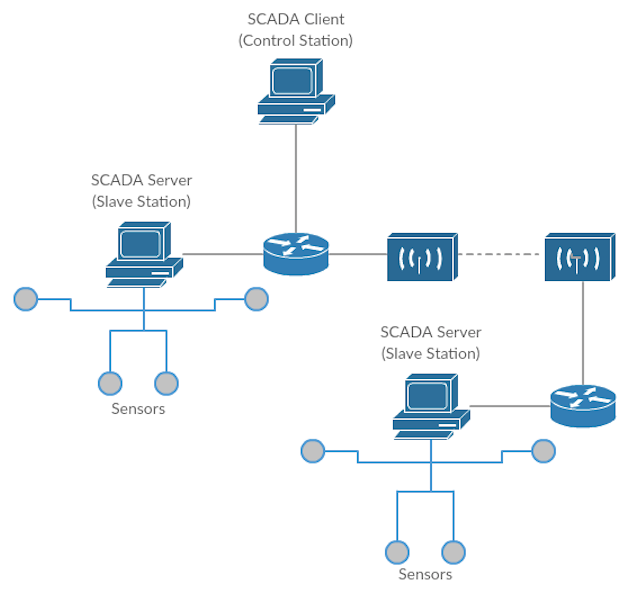
\includegraphics{scada}}
    \caption{Topológia SCADA systému}
\label{scada}
\end{figure}
Systémy slúžia na vzdialenú kontrolu a zber údajov. Využívajú sa v nich tzv. inteligentné merače - IED (Intelligent Electronic Devices). Jednotlivé zariadenia sú prepojené a vzájomne komunikujú cez aplikačnú zbernicu (fieldbus). Taktiež sú pripojené k riadiacemu centru, ktoré ich vzdialene kontroluje a ovláda. Ukážka prepojenia je na obrázku \ref{Fieldbus}. Vzdialenosť riadiach staníc (master) a koncových zariadení (slave) môže byť od niekoľkých metrov po tisíce kilometrov. Každé zariadenie môže obsahovať niekoľko rôznych senzorov, analógový vstup/výstup senzora, systém na komunikáciu s riadiacim počítačom a zariadeniami, a programovú pamäť\cite{SCADA}. \par
\begin{figure}[h]
    \centering
    \scalebox{0.6}{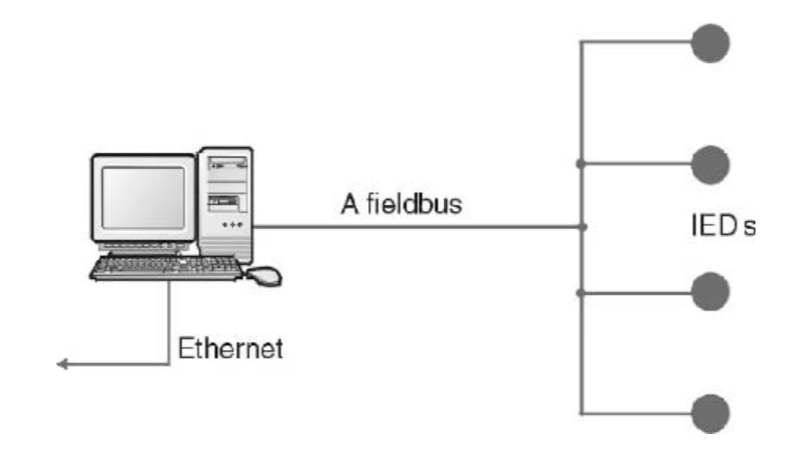
\includegraphics{Fieldbus}}
    \caption{Zapojenie zariadení v SCADA\cite{SCADA}}
\label{Fieldbus}
\end{figure}

\textbf{Výhody SCADA systémov sú:}
\begin{itemize}
\item Je potrebná minimálna kabeláž - oproti prvotným verziám SCADA systémov kedy sa nevyužívali IED zariadenia a každý senzor musel byť samostatne pripojený ku kontrolným staniciam
\item Prijímané dáta môžu obsahovať veľkú škálu informácií - seriové čísla, čísla modelu, informácie o inštalácií zariadenia (kedy bolo nainštalované a kým)
\item Zariadenia sú jednoduché na inštaláciu, prípadne výmenu
\item Celý systém potrebuje málo fyzického priestoru - jednotlivé koncové zariadenia sú relatívne malé
\end{itemize}
\textbf{Nevýhody sú:}
\begin{itemize}
\item Využívanie sofistikovanejších systémov je náročnejšie a vyžaduje lepšie vyškolený a kvalifikovaný personál
\item Ceny senzorov sú vyššie
\item Zariadenia sú závislé na komunikačnom systéme - je nutné aby podporovali rovnaký komunikačný protokol
\item Postupný prechod systémov nad IP vrstvu znižuje ich bezpečnosť\cite{SCADA}
\end{itemize}
\subsection{Komunikačné protokoly}
\tab Aby mohli medzi sebou koncové zariadenia a riadiaca stanica komunikovať, musia podporovať rovnaký spôsob komunikácie. Na to slúžia rôzne štandardizované protokoly, ktoré takúto komunikáciu popisujú. V tejto práci sa budem venovať dvom z nich. Konkrétne to sú protokoly IEC 60870-5-104 a DLMS/COSEM.
\subsubsection{IEC 60870-5-104}
\tab Protokol IEC 60870-5-104 je časť protokolu IEC 60870-5. IEC 60870-5 je komunikačný protokol a je súčasťou protokolu IEC 60870, ktorý je určený pre systémy diaľkového riadenia. IEC 60870-5 špecifikuje prenosové protokoly pre diaľkové ovládanie zariadení, ktoré slúžia k prenosu dát a riadeniu geograficky vzdialených procesov. Pozostáva z niekoľkých častí, z ktorých nás najviac zaujíma IEC 60870-5-104. Protokol IEC 60870-5-104 špecifikuje sieťový prístup pre IEC 60870-5-101. Protokol IEC 60870-5-101 je spoločná norma pre základné úlohy diaľkového ovládania. Jeho cieľom je zaistiť vzájomnú spoluprácu medzi jednotlivými (kompatibilnými) zariadeniami pre diaľkové riadenie. Tzn. že IEC 60870-5-101 špecifikuje mechanizmy prenosu a IEC 60870-5-104 stanovuje ich použitie v bežných komunikačných sieťach\cite{SCADA}\cite{Pekarek}.\par
Protokol IEC 60870-5-104 je umiestnený na aplikačnej vrstve modelu ISO/OSI. Špecifikácia IEC 60870-5-104 kombinuje aplikačnú časť protokolu IEC 60870-5-101 a prenosové funkcie poskytované TCP/IP. Protokol poskytuje funkcie pre prenos dat aplikačným funkciám užívateľského procesu. Prenášaná správa je vo formáte APDU (Application Protocol Data Unit). Je to tzv. aplikačná jednotka, ktorá pozostáva z dvoch častí - APCI (Application Protocol Control Information) a ASDU (Application Service Data Unit). APCI je záhlavie aplikačnej jednotky, ktoré určuje jej dĺžku, typ, sekvenčné čísla a pod. ASDU sú samotné prenášané dáta, tj. príkazy posielané medzi klientom a serverom. APDU správa môže mať pevnú alebo variabilnú dĺžku. Správa s pevnou dĺžkou neobsahuje ASDU časť. Formát rámca je ukázaný na obrázku \ref{APDU}.
\begin{figure}[h]
    \centering
    \scalebox{0.35}{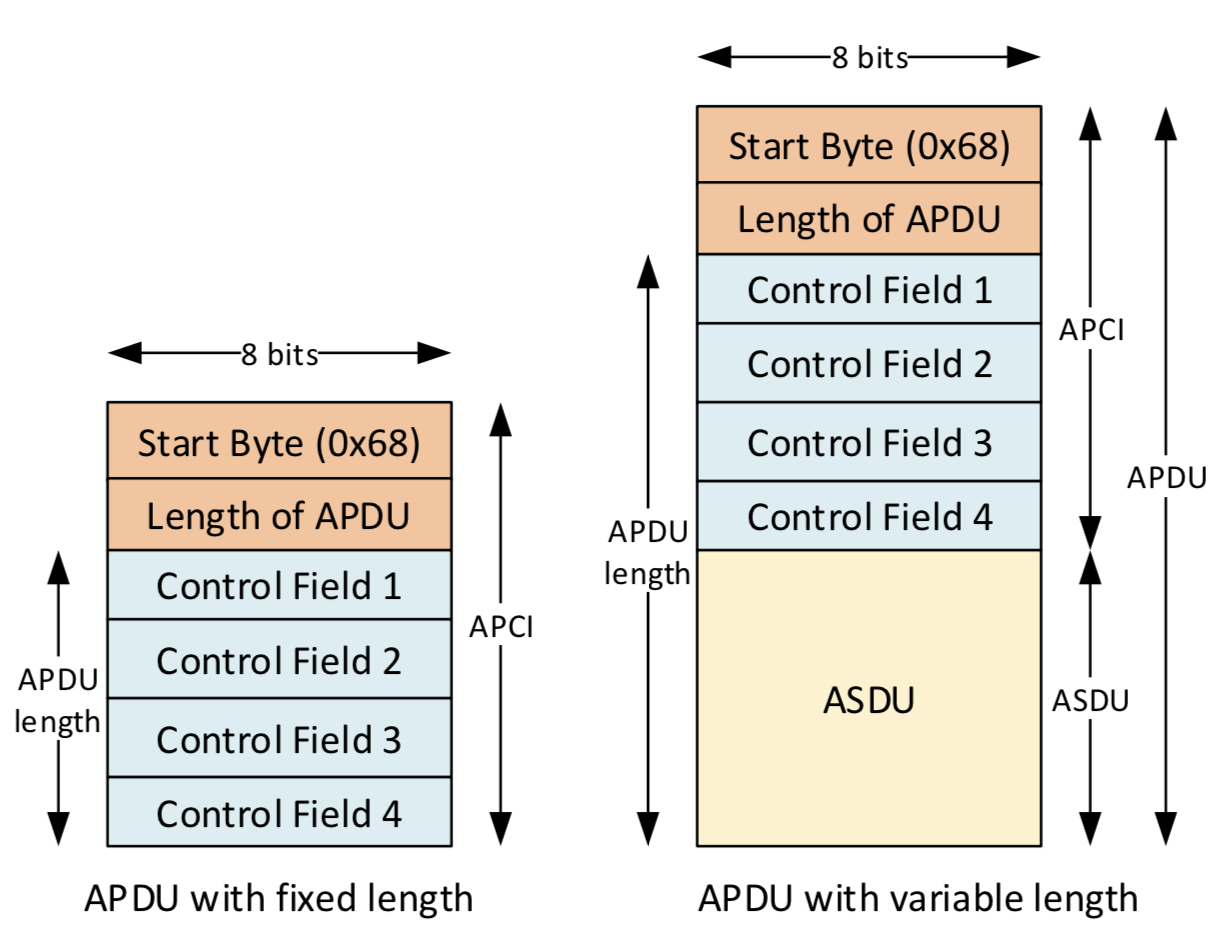
\includegraphics{APDU}}
    \caption{Formát APDU rámca\cite{iec}}
\label{APDU}
\end{figure}
Formát je určený poslednými dvoma bitmi prvého kontrolného poľa APCI časti (CF1). Štandard definuje tri typy rámcov, viď obrázok \ref{FrameFormat}.
\begin{figure}[h]
    \centering
    \scalebox{0.35}{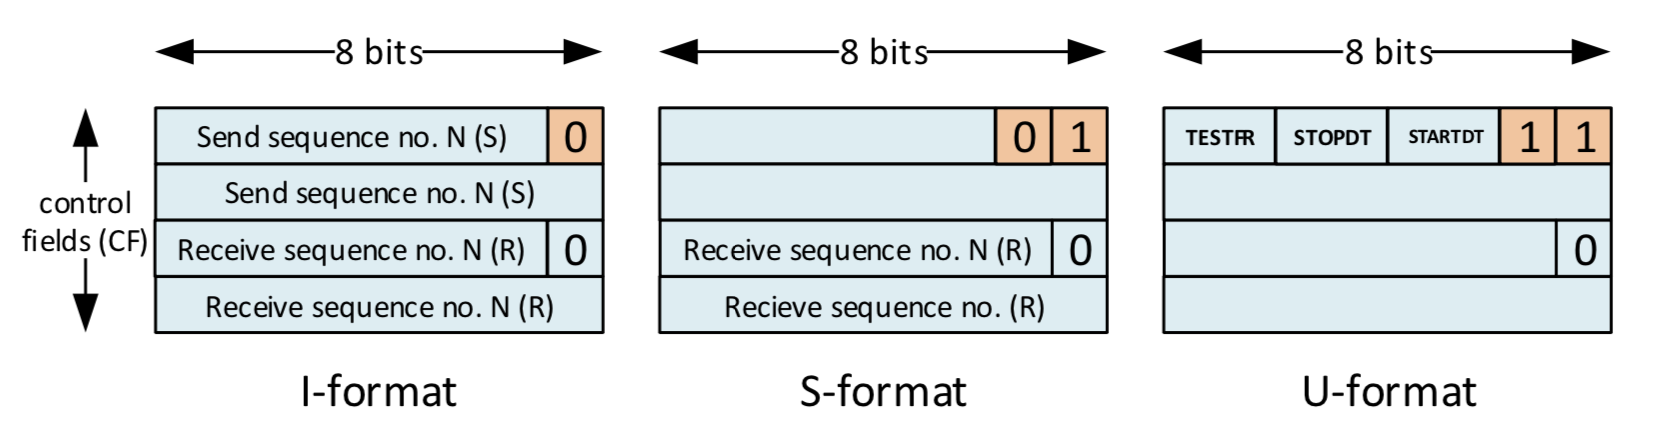
\includegraphics{FrameFormat}}
    \caption{Typy rámcov APDU\cite{iec}}
\label{FrameFormat}
\end{figure}
\begin{itemize}
\item I formát - je určený k bežnému prenosu dát medzi aplikačnými funkciami
\item S formát - je používaný pre dohľad nad prebiehajúcou komunikáciou
\item U formát - je určený k riadeniu samotnej komunikácie
\end{itemize}
\par
APCI vždy začína "štart bytom" s hodnotou 0x68. Za ňou nasleduje 8-bitové APDU a štyri 8-bitové kontrolné polia (CF). \par 
ASDU pozostáva z dvoch hlavných častí - identifikátor datovej jednotky (má vždy pevnú dĺžku šesť bytov) a dáta samotné, ktoré môžu pozostávať z jedného, alebo viacerých objektov. Identifikátor datovej jednotky definuje špecifický typ dát, poskytuje adresovanie na identifikáciu špecifickej identity dát a obsahuje dodatočné informácie ako napr. dôvod prenosu. Každé ASDU môže preniesť najviac 127 objektov. Na obrázku \ref{ASDU} je ukážka formátu ASDU\cite{iec}.
\begin{figure}[h]
    \centering
    \scalebox{0.4}{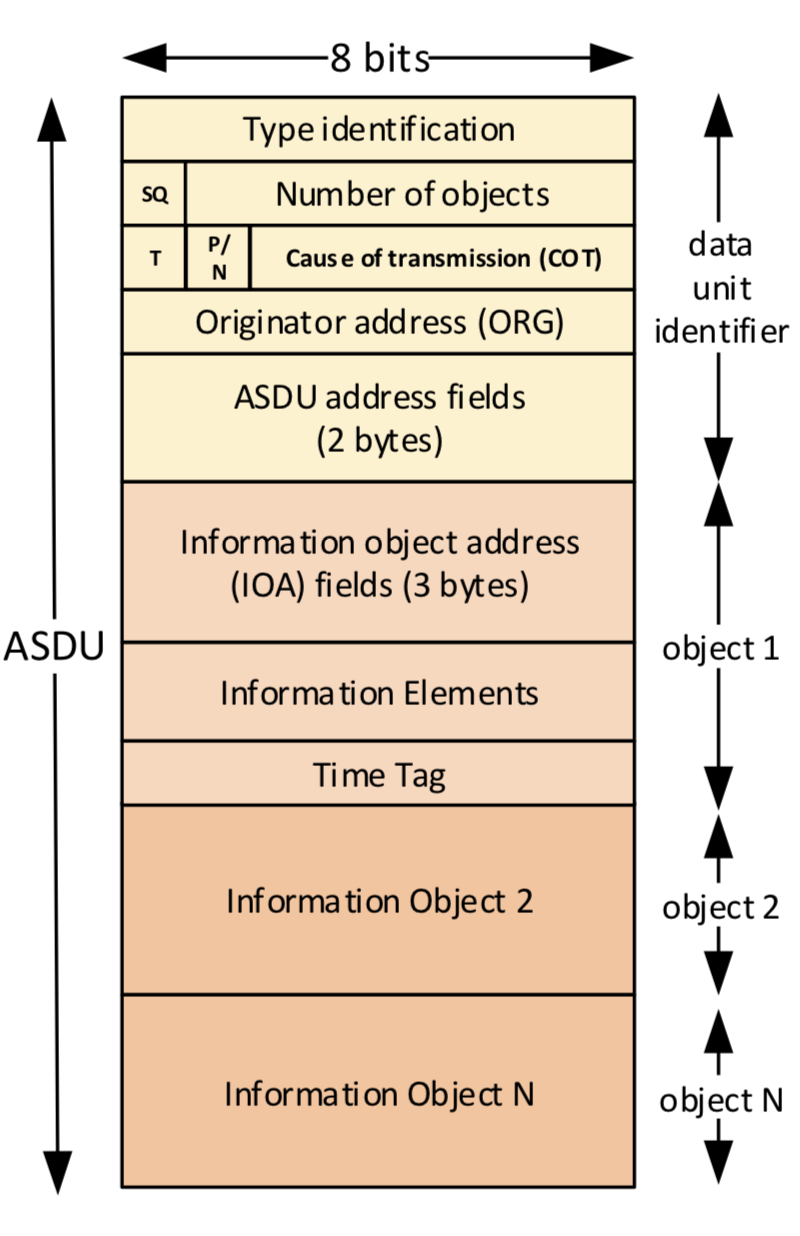
\includegraphics{ASDU}}
    \caption{Formát ASDU\cite{iec}}
\label{ASDU}
\end{figure}
\par
Riadenie prebieha pomocou niekoľkých príkazov - {\tt TESTFR}, {\tt STARTDT} a {\tt STOPDT}. {\tt STARDT} a {\tt STOPDT} sú príkazy používané riadiacimi stanicami na riadenie datového prenosu z riadenej stanice. Keď započne komunikácia, prenos dát nie je ešte povolený. Riadiaca stanica musí povoliť datový prenos odoslaním príkazu {\tt STARTDT act} (activate). Riadená stanica odpovie príkazom {\tt STARTDT con} (confirm). Ak nie je príkaz {\tt STARTDT} potvrdený, riadiaca stanica automaticky ukončí spojenie. Príkaz {\tt STARTDT} posiela iba riadiaca stanica a je odoslaný iba raz, po prvotnej inicializácií spojenia. Po povolení prenosu dát prebieha ľubovolná komunikácia medzi riadiacou a riadenou stanicou. Spojenie sa ukončuje príkazom {\tt STOPDT}.\par
Komunikácia vždy pozostáva medzi riadiacim (master) a riadeným (slave) systémom. Riadiaci systém inicializuje spojenie, začína a ukončuje výmenu aplikačných dát. Ukončenie komunikácie môže iniciovať riadiaca, ale aj riadená stanica. Riadená stanica (server) načúva na porte 2404 na príkazy od riadiacej stanice (klienta). Riadiaca stanica môže naraz komunikovať s viacerými riadenými stanicami\cite{iec}\cite{Pekarek}.
\subsubsection{DLMS/COSEM}
\tab Protokol DLMS/COSEM je, podobne ako protokol IEC 60870, súbor štandardov pre výmenu údajov o spotrebe v energetike. Protokol pozostáva z niekoľkých častí, pričom každá špecifikuje určitú časť problematiky, ktorú protokol rieši. Prvá časť, DLMS (Device Language Message Specification) je špecifikácia aplikačnej vrstvynezávislá od nižších vrstiev, vytvorená na podporu prenosu zpráv do a z vzdialených (energetických) zariadení. Cieľom je poskytnúť interoperabilné prostredie pre výmenu dát. Špecifikácia podporuje funkcie na vzdialené čítanie a nastavovanie hodnôt pre všetky odvetvia energetiky (elektrárne, vodárne, teplárne, atp.). DLMS je používané na popis rozhrania tried jednotlivých objektov spolu s ich atribútmi. Špecifikácia je podobná protokolu IEC 62056, ten je ale zameraný na meranie spotreby elektrickej energie na rozdiel od DLMS, ktorý je použiteľný na všetky energetické odvetvia. Druhá časť protokolu, COSEM (Companion Specification for Energy Metering) je rozhranie modelu komunikujúceho zariadenia na meranie energetickej spotreby, ktoré poskytuje pohľad na funkčnosť dostupnú cez komunikačné rozhranie. Poskytuje taktiež sémantiku na aplikáciu jednotlivých meraní. COSEM model je založený na objektovo-orientovanom prístupe. Instancia COSEM rozhrania sa nazýva {\tt COSEM interface object}. Sada jednotlivých objektov v logických zariadeniach fyzického zariadenia modeluje funkcionalitu meracích zariadení rovnako ako je to možné vidieť v jeho komunikačnom rozhraní\cite{dlmscosem}. \par
Model reprezentuje meracie zariadenie ako server využívaný aplikáciami klienta. Aplikácie slúžia na získavanie dát, poskytovanie riadiacich informácií a spušťanie funkcií objektu pomocou riadeného prístupu k jeho atribútom a špecifickým metódam jednotlivých typov objektov. \par
\begin{figure}[H]
    \centering
    \scalebox{0.3}{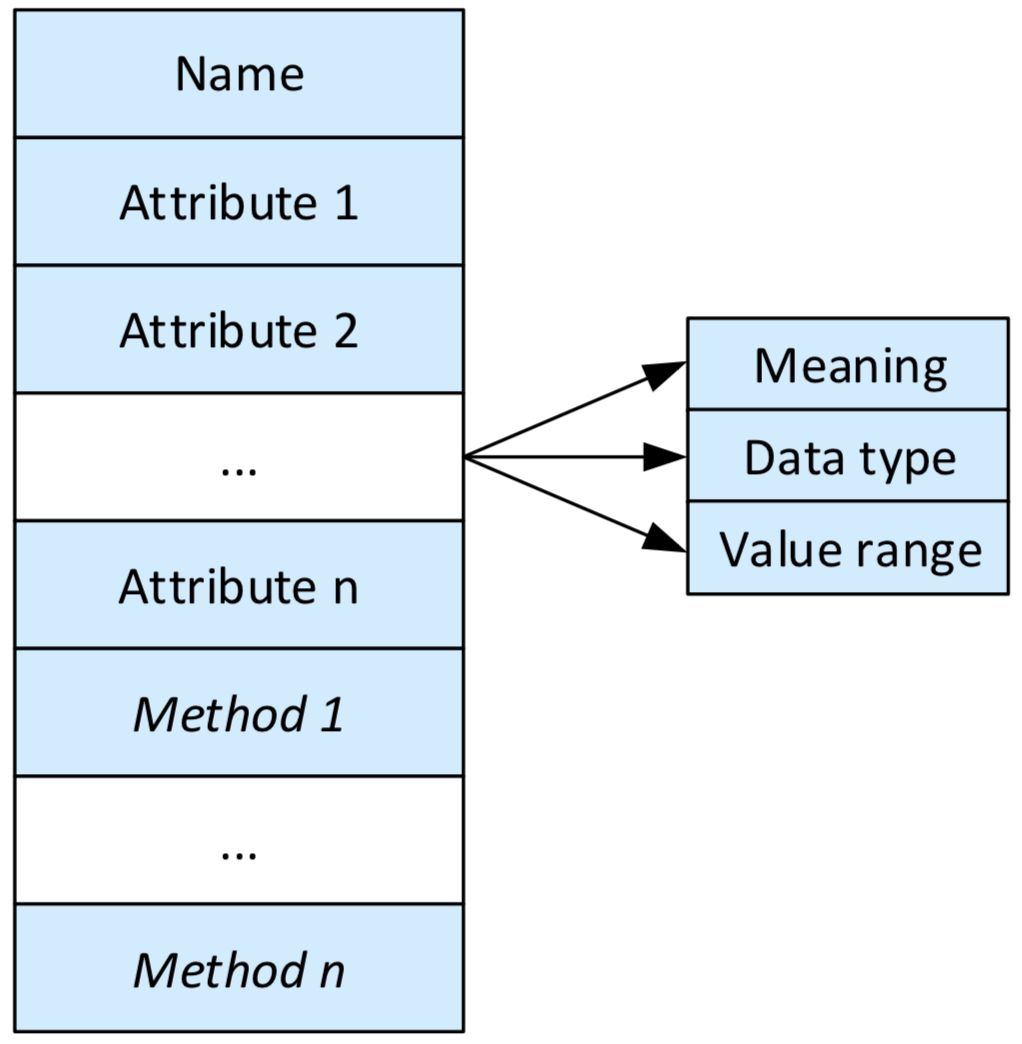
\includegraphics{dlmsattribute}}
    \caption{COSEM objekt\cite{dlmscosem}}
\label{dlmsattribute}
\end{figure}
COSEM modeluje fyzické zariadenie ako súbor logických zariadení, pričom každé má svoj jednoznačný identifikátor. Identifikátor určuje typ (funkcionalitu) daného zariadenia. Každé zariadenie môže byť jednoznačne identifikované pomocou jeho logického mena (OBIS kódom). Ide o šesť 8-bitových číslic. Informácie obsiahnuté v jednotlivých logických zariadeniach sú modelované objektami rozhrania. Objekty rozhrania sú špecifické pre danú doménu merania spolu s ich atribútmi a metódami. V atribútoch sú usporiadané informácie, ktoré daný objekt uchováva. Vlastnosti objektu sú určené pomocou hodnôt atribútov. Každý atribút pozostáva z typu, hodnoty a určenia. Ukážka objektu je na obrázku \ref{dlmsattribute}. \par
Prvý atribút každého objektu je jeho logické meno, ktoré slúži na identifikáciu objektu. Objekty, ktoré majú rovnakú charakteristiku sú generalizované a identifikované pomocou ID ich triedy (class\_id). Vzťah medzi šablónami a rozhraniami tried je ukázaný na obrázku \ref{dlmsobject}. Štandard protokolu definuje približne 70 rozhraní tried pričom každé je určené jeho menom, ID triedy a verziou.
\begin{figure}[H]
    \centering
    \scalebox{0.4}{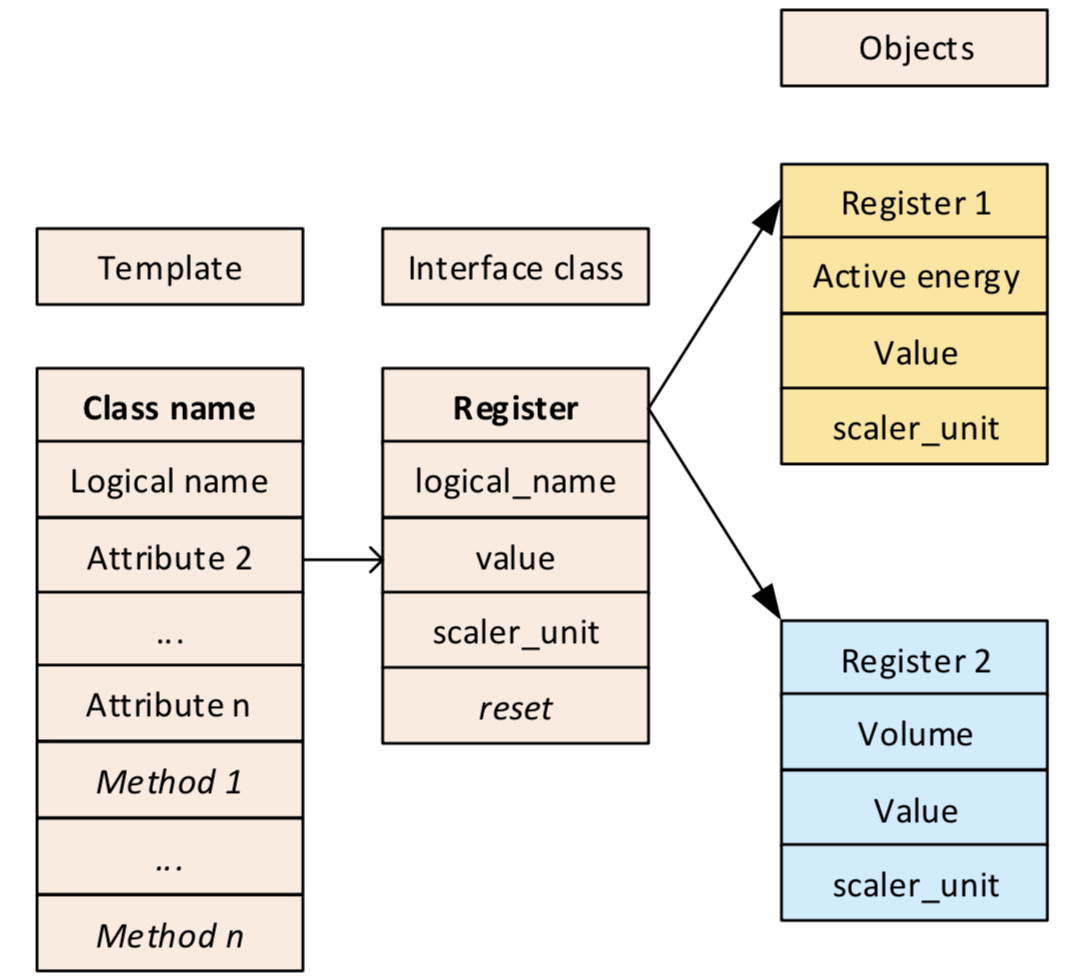
\includegraphics{dlmsobject}}
    \caption{Šablóny a rozhrania tried\cite{dlmscosem}}
\label{dlmsobject}
\end{figure}
Jednotlivé metódy umožňujú identifikáciu, vyhľadávanie a interpretáciu informácií uchovávaných v objektoch meracích zariadení\cite{dlmscosem}\cite{Horych}. \par
\begin{figure}[H]
    \centering
    \scalebox{0.6}{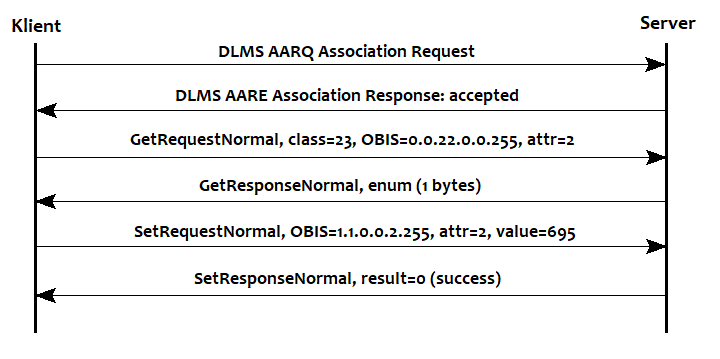
\includegraphics{comm.png}}
    \caption{Komunikácia protokolu DLMS/COSEM}
\label{dlmscom}
\end{figure}
Na obrázku \ref{dlmscom} je ukážka komunikácie protokolu DLMS/COSEM medzi klientom a serverom. Ukážka obsahuje niekoľko bežných príkazov. Ako prvé nnačítanie informácií o jednotlivých pripojených meračoch (Association Request/Response), tento príkaz je vždy zasielaný ako prvý na začiatku komunikácie. Druhá je žiadosť o navrátenie hodnoty druhého atribútu objektu s OBIS kódom 0.0.22.0.0.255. Ide o hodnotu prenosovej rýchlosti (baudrate) objektu typu {\tt IecHdlcSetup}. Nakoniec je zaslaný príkaz na nastavenie druhého atribútu objektu s OBIS kódom 1.1.0.0.2.255. Je to atribút nesúci údaje o spotrebe v objekte typu {\tt Data}. \par
Dáta prenášané protokolom DLMS/COSEM sú väčšinou zapúzdrené do tzv. HDLC rámca definovaného štandardom ISO/IEC 13239\cite{dlmscosem}. Štandard používa formát HDLC rámca typu 3, ukážka je na obrázku \ref{hdlc_frame}.
\begin{figure}[H]
    \centering
    \scalebox{0.6}{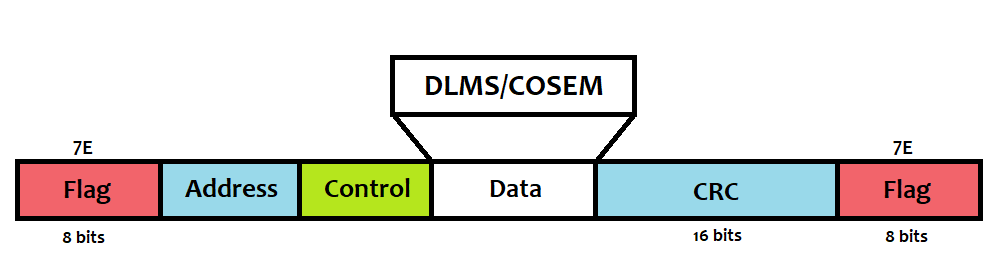
\includegraphics{hdlc_frame.png}}
    \caption{HDLC rámec}
\label{hdlc_frame}
\end{figure} \par
Rámec neobsahuje informačné pole, kontrolnú sekvenciu hlavičky (HCS) iba kontrolnú sekvenciu rámca. Prvé štyri bity slúžia na identifikáciu HDLC rámca. Pre DLMS je to 1010 (0xA). Kontrolné pole (CTRL) označuje typ príkazu alebo odpovede a obsahuje patričné sekvenčné číslo. Ukážka kontrolného poľa je na obrázku \ref{ctrl}.
\begin{figure}[H]
    \centering
    \scalebox{0.55}{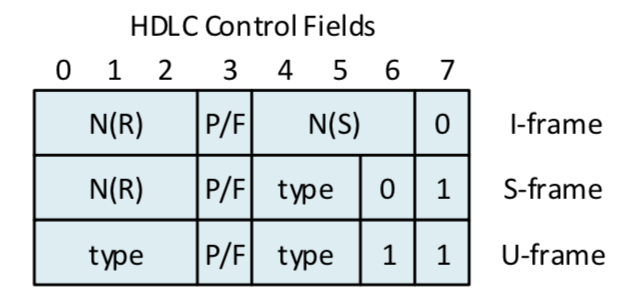
\includegraphics{ctrl}}
    \caption{Kontrolné pole HDLC rámca\cite{dlmscosem}}
\label{ctrl}
\end{figure} \par
Sú tri typy rámcov:
\begin{itemize}
\item I formát - informačný (information), prenáša užívateľské dáta zo sieťovej vrstvy 
\item S formát - kontrolný (supervisory), je používaný na kontrolu datového toku a chýb. Neobsahuje informačné polia. Používajú sa tri typy kontrolného rámca:
\begin{itemize}
\item 00: Pripravený na prijímanie, RR (Receive ready)
\item 01: Prijímanie, nie čítanie, RNR (Receive not read)
\item 10: Zamietnuté, REJ (Reject)
\item 11: Selektívne domietnutie, SREJ (Selective reject)
\end{itemize}
\item U formát - nečíslovaný (unnumbered) je používaný na správu odkazov (nastavenie režimu, zotavenie) a môže byť tiež použitý na prenos užívatľských dát
\end{itemize} \par
Pre DLMS/COSEM je potrebné parsovanie rámcov na identifikáciu vonkajšieho zapúzdrenia. HDLC môže byť identifikované začiatočným a koncovým príznakom (flag), ktorý má hodnotu 0x7e\cite{dlmscosem}.











